\subsection{Codelenses} \label{codelenses}
Codelenses are visual studio code features which is also common to many other IDEs. The idea is to display metainformation about certain pieces of codes, for instance classes and methods. In visual studio code this is done  by adding an additional line of text to the editor whereever a code lense should  be placed. \newline

Since this can be used to quickly gain a deeper understanding of a codebase, it was decided to integrate this feature. Another reason was that it is widespread in different IDEs, so that programmers have become acostumed to it. \newline

\begin{figure}[H]
	\centering
	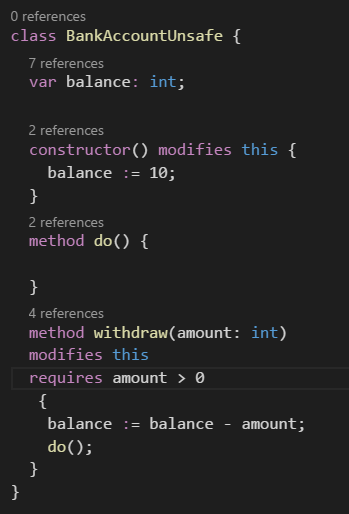
\includegraphics[width=0.5\textwidth]{img/codelensesClosed}
	\caption{Code Lenses used with Dafny}
	\label{fig:codelensesclosed}
\end{figure}

The first decision to be made was for which elements in the code codelenses should be displayed. The adeoff here is to  provide enough information to work comfortably with the codebase and not to clutter the workspace with codelenses. It was decided to display codelenses for classes, methods (including constructors) and fields, since they tend to have a wide scope in the codebases. \newline
A second consideration was which information should be displayed in the codelens. When codelenses are language specific and do not for instance stem from a plugin which displays code metrics are similar, usually references and usages of the element are displayed. Since this allows the programmer to gain a deeper understanding of control flow and regions affected by refactorings, it was decided to display this information also for the Dafny plugin. Codelenses also allow commands to be executed when clicked upon, a logical conclusion is to implement go to reference when a reference in a codelens is clicked.\newline

\begin{figure}[H]
	\centering
	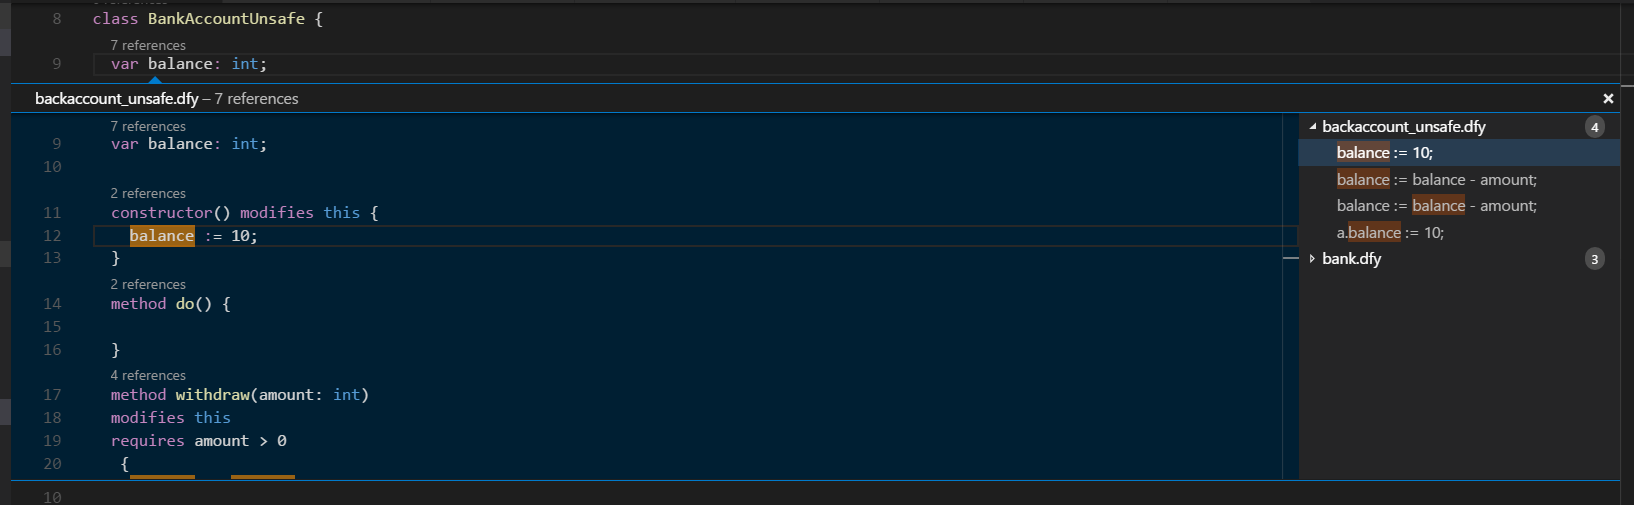
\includegraphics[width=1\textwidth]{img/codelensesExpanded}
	\caption{Expanded codelens showing the references to the field balance}
	\label{fig:codelensesexpanded}
\end{figure}

The only challenging aspect when implementing this feature is that references can't be determined via a simple text search, since different classes could have member with the same name. To only display unambiguous references, the search has to be done via the fully qualified domain name of the symbol. Since information about references is needed often, all references are determined by the DafnyServer and returned together with the symbolinformation to the symbolservice. This allows for simple processing in the language server itself and the references are updated in real time, since the symbolservice refreshes the symbols for a file when it is changed. Off course also the filepath belonging to the file in which the reference occurs is returned by the symbolservice. This is needed when a reference is a file external to the defining one and the go to reference command is invoked.\newline
When given locations of the references, it is possible to let visual studio code highlight them in the preview window which opens when a codelens is expanded. Visual studio code also groups references according to the filepath in the location, so the programmer gets to see a map of all references ordered by containing file to the right of preview window and can quickly navigating to them.

 \subsection{Code Completion} \label{codecompletion}
 Code completion has become a standard feature for IDEs. Microsoft calls it Intellisense in its products. It enables programmers to rapidly write code without having to keep all definitions in mind. Usually, when the programmer starts typing, a little popup appears where the programmer can choose options that complete the code he is currently writing. \newline
 
 Since this is arguably one of the most helpful features in IDEs, the implementation thereof was paramount to the completion of this project. \newline
 
 \begin{figure}[H]
 	\centering
 	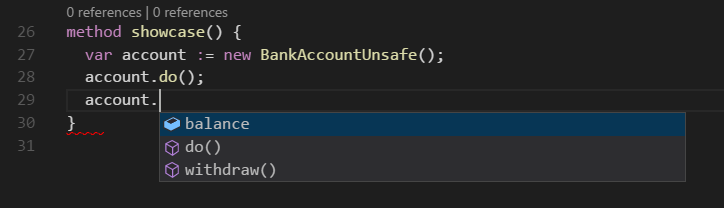
\includegraphics[width=1\textwidth]{img/codeCompletionOverview}
 	\caption{Popup with completion options}
 	\label{fig:codecompletionoverview}
 \end{figure}
 
 There are several different considerations when implementing code completion in a language server. The first one is to define which typed characters should trigger a completion request. Ideally, an IDE supports the programmer with completion regardless of the current context. Next to performance, another reason to narrow down the trigger selection is that not all contexts warrant meaningful suggestions for completion. In this project, a pragmatic approach was chosen where completion is triggered when ever a "." is typed, a situation where the programmer usually wants to access a member of an element. Since there is usually a designator present before the ".", there exists also enough knowledge about the current context to offer meaningful options. \newline
 In order to support this, the symbol service stores all variable declarations so the plugin knows about the type of all expressions that can be followed by a ".". The completion request comes with a position in the current file as an argument, so the first task is to resolve the expression and find out the fully qualified name of each element. The language server then searches the symbol service for all members that are defined in the class with that fully qualified name and sends them back as completion suggestions. \newline
 Visual Studio Code then handles all further actions, for instance, once the popup is displayed and the programmer continues to type, it removes all suggestions that don't start with the typed characters. It is also possible to display further information regarding the suggestions. The plugin already details if the completion is a field or a method, which Visual Studio Code provides own icons for. When the suggestion is a method, the preconditions, if any, are also displayed, so the programmer already knows the constraints he is writing under. \newline
 
 \begin{figure}[H]
	\centering
	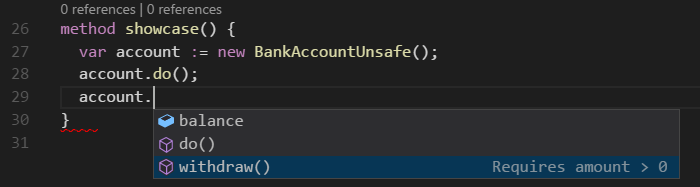
\includegraphics[width=1\textwidth]{img/codeCompletionMethod}
	\caption{Suggestion displaying precondition}
	\label{fig:codecompletionmethod}
\end{figure}

The implementation is straightforward, as the symbol service already provides ways to resolve the fully qualified name of an expression and if it as an alias for an element of a class, all therein defined methods and fields can simply be collected. The method and field symbols in the symbol services also contain all additional information which is displayed in the popup. Possible improvements in the completion feature would be support of built in methods and functions and also offer context aware completion when the programmer starts to type an identifier. 

\subsection{Go to Definition} \label{gotodefinition}
Another common feature in modern IDEs is go to definition. It enables the programmer to quickly jump to the definition of a code element he is currently working with to gain further insight about it. This can usually be done either via hotkey for the current cursor position or an option when opening the context menu via a right click, Visual Studio Code offers both ways.\newline
Since, similar to code lenses, this is a feature which is elemental to all modern IDEs and provides great overview over a project, the implementation of this feature had a high priority in this project. \newline
 \begin{figure}[H]
	\centering
	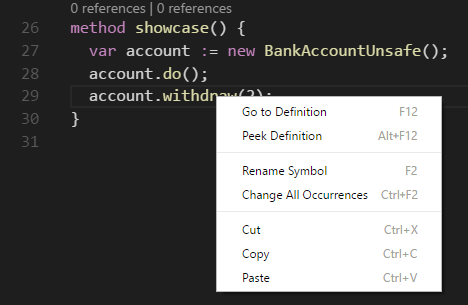
\includegraphics[width=0.5\textwidth]{img/goToDefinition}
	\caption{The Definition Features}
	\label{fig:gotodefinition}
\end{figure}
The language server protocol offers an on definition request, which has URI of the file and the position for which a definition is requested as parameters. The plugin language server then first tries to resolve the word at the position which could lead to a definition. When a word could be resolved, the plugin tries to determine if the expression is an alias for an element of a class or if it stands for an access of a member of one. If this is the case, the fully qualified name of the symbol can be determined via the symbol service, as it stores information about all definitions and declarations. The plugin than finds the unambigious definition via the fully qualified name and responds with the location of that definition. This also works if the definition is in an external file in the same workspace. \newline
If, for whatever reason, the fully qualified name cannot be determined, the plugin tries to match the selected word with any symbol cached in the symbol service. This approach only works as best effort though, as different classes could defines methods with the same name for example. If no match is found at all, no definition is provided. \newline
Visual Studio Code offers to options when searching for definitions, either go to definition which immideatly opens the returned location in an editor or peek definition, which shows the definition in a little overlay. \newline
 \begin{figure}[H]
	\centering
	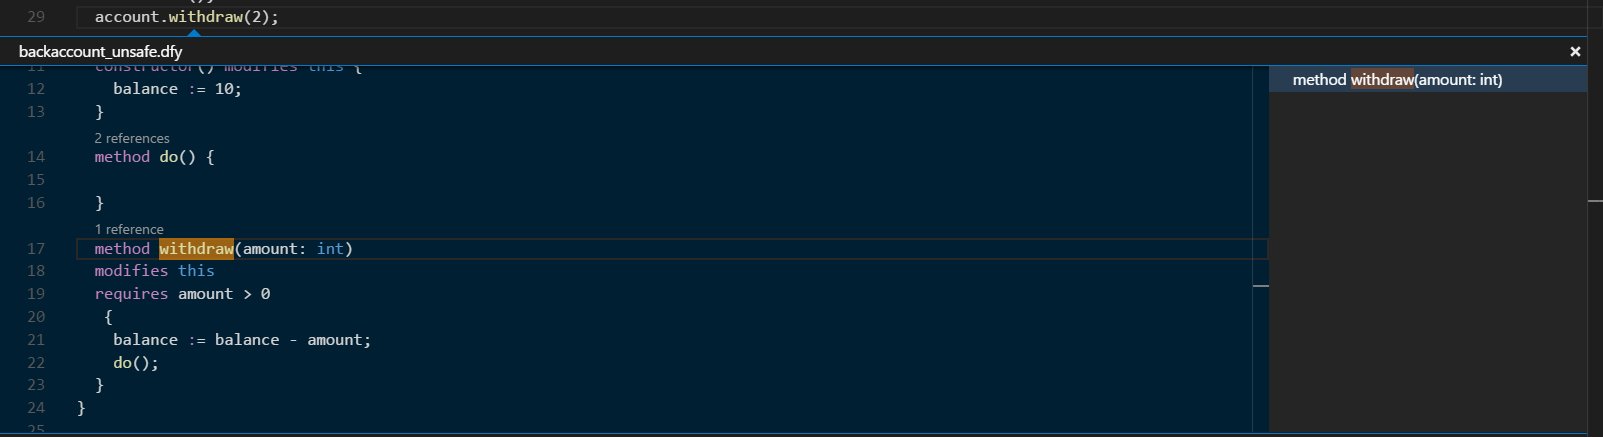
\includegraphics[width=1\textwidth]{img/goToDefinitionPeek}
	\caption{Overlay of peeked definition}
	\label{fig:gotodefinitionpeek}
\end{figure}
Extensions to this feature could be a context aware heuristic when a fully qualified name cannot be determined where for instance the current and nearby files are preferred when searching for definitions. Also, when polymorphism comes into play and the actual implementation cannot be determined, at the current state the first possibility is returned. The could be enhanced by offering all possible definitions.


\subsection{Rename Element} \label{renameelement}
Rename element is a feature essential to refactoring. It is widespread in IDEs and allows to quickly make code better readable Visual Studio Code offers built in support for renaming either via a hotkey or the context menu. \newline
Because of its importance in refactoring, which is one of the most important tasks when programming, implementing this feature belongs to the core scope of this project. \newline
The language server protocol, as with many other features, offers a request for renaming with the URI of the file in which the command was invoked and the position belonging to the command. Additionally, the new name the element should have is also given as an argument. The protocol expects a collection of textedit commands, which entail an URI of file, and ranges in that file which should be replaced with a word. \newline
As often with the language server protocol, the first step when implementing the feature is to determine the element at the position which is given as an argument. When the position can be resolved to a meaningful word, the plugin tries to determine if it is either an alias for an element of a class, or a member of class, for instance a field or a method. If it can do so with absolutely certainty, the fully qualified name of that element is obtained. The next step is trivial, since the symbol service already caches all references to a symbol, information which it gained through the DafnyServer. The plugin can simply build textedits out of all references, since the reference already contain all necessary information such as the containing file and their position therein. This therefor also works across multiple files which reference the same element, as long they are open in the same workspace. Those textedits are then returned from the language server to Visual Studio Code, which does all the actual replacing. \newline
  \begin{figure}[H]
 	\centering
 	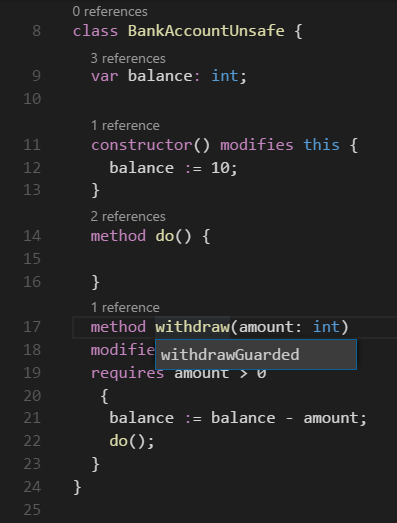
\includegraphics[width=0.5\textwidth]{img/rename}
 	\caption{Renaming an element in Visual Studio Code}
 	\label{fig:rename}
 \end{figure}
Since this feature acutally changes code that is worked with, the implementation must be very robust and failsafe. Thus, it was implemented very defensive. It the location of a requested renaming cannot be resolved to a meaningful word, the request is ended without dictating any changes. The same hold if a word can resolved, but it cannot be matched to a fully qualified name. In this case, possible references could be ambigious, so no action should be taken. To further limit the possibility for failure, the scope for this feature is very small. The current stand only allows for renaming of class members susch as fileds and methods, since these can be resolved with absolute certainty.\newline
When extending this feature, if would be benefical to also be able to rename local variables for instance. To do this, the symbol informtation which the DafnyServer returns to the symbol service would have to be enriched with detailed scope information to allow being able to exactly say which regions are prone to renamings and which are not. 
\subsection{Quick Fixes} \label{quickfixes}
Quick Fixes are a versaile feature in IDEs which basically allow to do any manipulation to code. Usually they are offered as reactions to diagnostics which were provided earlier. A simple example would be implementing a spell checker this way, offering to replace a wrongly written word with the correct spelling. \newline
Since this feature has no clear implementation guideline, and the plugin designer can implement almost anything that he likes this way, this was an obvious place to implement Dafny specific feature in the plugin. \newline
They this works in Visual Studio Code is, when the diagnostic stage for the file has been completed, where all things such as compiler warnings or custom warnings are generated,  a new request is fired at the language server. This request holds a collection of all diagnostics on the current file and the the language is free to either do nothing are provide commands for some diagnostics in the collection which often aime to resolve the shortcomings detailed by the diagnostic. \newline
  \begin{figure}[H]
	\centering
	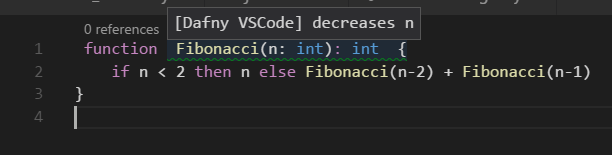
\includegraphics[width=1\textwidth]{img/diagnostic}
	\caption{Visual Studio Code displays a diagnostic}
	\label{fig:diagnostic}
\end{figure}
The current stand of the projects offers two code fixes to resolve Dafny specific diagnostics. \newline
The first one is a common situation where a programmer fails to capture his intention that a variable should either decrease or increase a variable when working with recursion or loops. The remedy is simple, a decrease guard with the variable in question must be added at the correct location. \newline
  \begin{figure}[H]
	\centering
	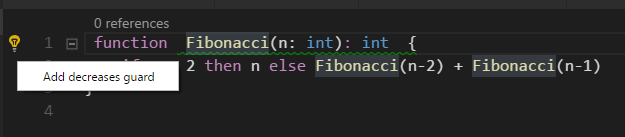
\includegraphics[width=1\textwidth]{img/decreaseGuard}
	\caption{Offering a code fix to add a guard}
	\label{fig:decreaseguard}
\end{figure}
This situation can easily be identified through the message within the diagnostic, since Dafny always gives this message in the same format. The expression that has to be decreased can also easily be parsed out of this message. A little more difficult is the placement of the guard, the implementation tries to find the first block in which the variable is not in scope anymore. The guard is then inserted before the block containing the first usage is used. \newline
  \begin{figure}[H]
	\centering
	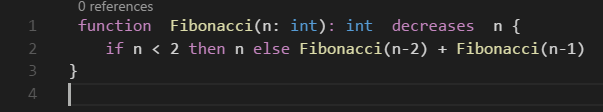
\includegraphics[width=1\textwidth]{img/decreaseGuardApplied}
	\caption{Programm after the code fix}
	\label{fig:decreaseguardapplied}
\end{figure}
The second code fix the plugin is offered is very similar, but this time the constraint is that an object may be null when it should not. The situtation again is easily detected through the message in the diagnostic, and also the expression which should not be null can be parsed through it.
  \begin{figure}[H]
	\centering
	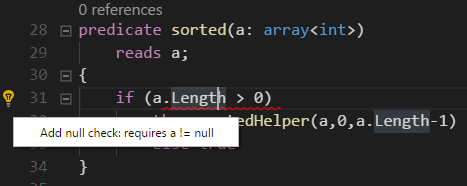
\includegraphics[width=1\textwidth]{img/nullCheck}
	\caption{It should be made sure that an element is not null}
	\label{fig:nullcheck}
\end{figure}
Also the search for the insertion position works very similary. It then inserts the constraint in form of a precondition of the sourrunding element. \newline
  \begin{figure}[H]
	\centering
	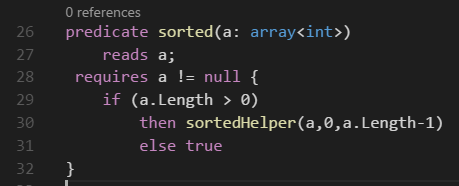
\includegraphics[width=1\textwidth]{img/nullCheckApplied}
	\caption{The precondition has been added}
	\label{fig:nullcheckapplied}
\end{figure}
At the current stand, only these two code fixes are implemented, the possible extensions are legion. 